\section{Analysis of different payment methods}

To revisit the concept from the introduction, the prerequisites have to be specified first:

\begin{enumerate}
    \item A potential customer Alice, who owns an electric car and wants to purchase electricity to charge it overnight.
    \item A supplier Bob, who owns a smart electrical socket, wants to sell electricity.
    \item Alice and Bob do not meet, Alice does not trust Bob to supply the electricity she paid for, Bob does not trust Alice to not wrongfully revert the payment after the electricity has been supplied. It has to be assumed that there are bad actors, who want to steal from the other party (in the form of monetary value or electricity).
    \item For all calculations throughout this thesis the following values are assumed:
    \begin{enumerate}
        \item Charging power: 3.7 kW
        \item Electricity price: 0.3 \euro/kWh
        \item Total transferred energy: 40 kWh
        \item Charging duration: 11 hours
        \item Electricity cost: 12\euro
        \item Price for the customer: 18\euro{} (profit margin of 50\%)
    \end{enumerate}
\end{enumerate}

The objective of this chapter is to evaluate which payment method is suited best for the described use case. Next, the goals of the M2M payment system have to be defined:

\begin{enumerate}
    \item Value has to be transferred from Alice to Bob.
    \item Electricity has to be supplied in return for a payment, whereby the risk or impact of not getting electricity in return has to be minimal.
    \item Alice needs to be able to stop paying for electricity when it's not longer needed, e.g. when the battery is fully charged, without overpaying.
    \item Bob should only start supplying electricity after a valid payment was received and thus the risk of losing electricity is minimized.
    \item Value should be transferred from Alice to Bob at least once per minute, to continuously pay for electricity to reduce risk, but transaction costs should stay at a minimum at the same time. For this thesis a payment interval of 15 seconds is assumed resulting in 0.007\euro{} per payment.
\end{enumerate}

Now that the requirements are defined it can be discussed, which payment method should be implemented on the prototype. In the following paragraph the advantages and disadvantages of traditional payment methods, established electronic and online payments and cryptocurrencies are compared.
\\\\
The simplest form of monetary value is cash, it could be imagined that money could be paid through a coin slot and electricity would be returned as a result. Unfortunately it's not suitable for this use case, as the risk of not receiving any electricity in return for the customer and the risk of theft for the supplier, e.g. someone violently stealing the cash, is too high.
\\\\
Traditional electronic or online payments like VISA or PayPal pose a low risk of theft for the buyer because of customer protection methods, unfortunately the risk for the seller is non-negligible, e.g. in the form of credit card fraud or customer protection exploitation. Another disadvantage are high fees, PayPal, for example, has a pricing of 0.10\euro{} + 10\% for micro-transactions\cite{paypal-fees} and wouldn't be economically feasible for the predefined goals. The key strength are fast, near-instant transaction times.
\\\\
Cryptocurrency payments have some major advantages over the previously analyzed payment methods. Compared to electronic and online payments, fees are low because they are fixed, not variable. Some cryptocurrencies even work without any fees at all. Payments can be broken down into fractions, as mentioned above with payment intervals of a minute or less. Because all payments are immutable the supplier has no risk, the customer risks just losing a less than one cent for a first payment. One of the biggest disadvantages of cryptocurrencies for M2M payments are long transaction times, but as the technology is still in its infancy, this might change in the future.
\\\\
Over a thousand different cryptocurrencies exist and every one of them has their own rules that can drastically differ from the next one. Each underlying blockchain technology has their benefits and drawbacks. In the next paragraph some of these digital currencies will be evaluated whether or not they are suitable to reach the set goals.
\\\\
Because Bitcoin is the earliest cryptocurrency, it suffers from problems other cryptocurrencies could improve upon. As demonstrated in figure \ref{fig:BitcoinConfirmationTime}, scalability is one of these issues. The block time is 10 minutes\cite{bitcoin-whitepaper} and during peak times the average confirmation time can take more than two hours. Thus bitcoin should not be considered for this use case.
\\\\
Ethereum has a block time of 15 seconds. At the time of writing the fee to be included in the next block is 0.01\euro\cite{ethereum-fee}. In this case the transaction would be fast enough to meet the goal of 4 transactions per minute, but the transaction cost would exceed the payment, raising the total price as much as 143\%.
\\\\
\begin{figure}[H]
    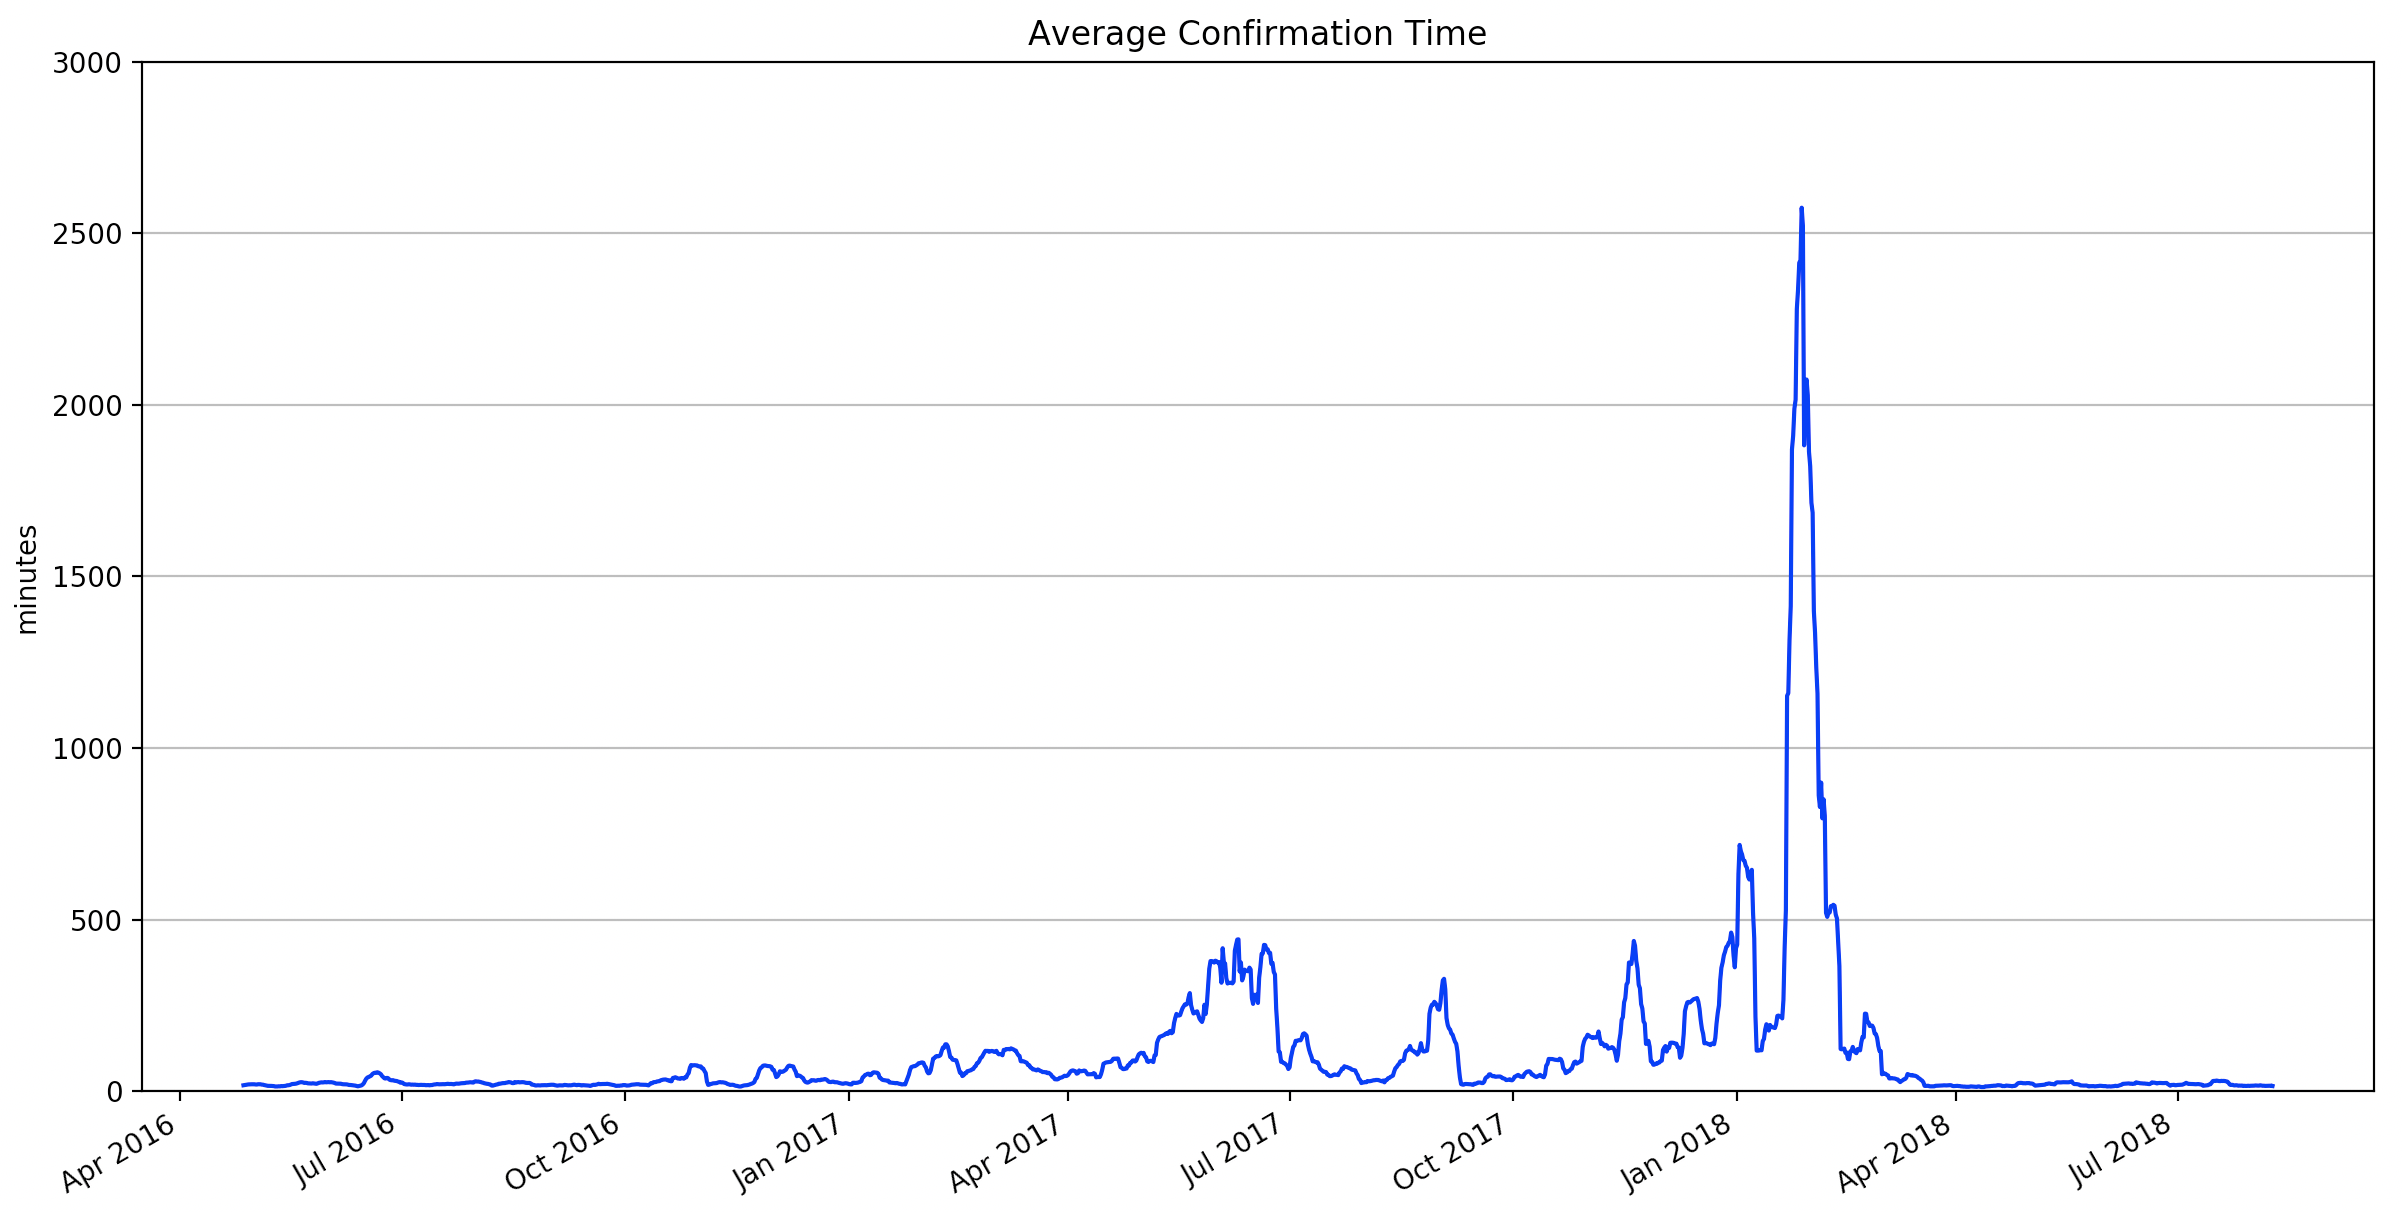
\includegraphics[width=\textwidth]{img/average-confirmation-time.png}
    \caption{Average confirmation time of a transaction on the Bitcoin blockchain\cite{btc-conf-time}}
    \label{fig:BitcoinConfirmationTime}
\end{figure}
\leavevmode
\\\\
As mentioned above there are some cryptocurrencies that work without any fees that are worth to be considered. One of these currencies is IOTA. It was designed especially with M2M payments in mind and the underlying technology, called Tangle, differs from traditional blockchains. The way it works is that before someones transaction can be validated, they need to validate other transactions first\cite{tangle}. In theory, this makes the network scale especially well — the more transactions are broadcasted, the shorter the transaction times get. In practice, transaction times are at 2.6 minutes at the time of writing\cite{iota-time}.
\\\\
Another feeless cryptocurrency is called Nano, formerly known as RaiBlocks. It's built upon a technology called block-lettuce. Each account on the network is an independent blockchain which can update itself asynchronously from the rest of the accounts. This makes Nano not only have zero transaction costs but also allows it to have transaction times of less than a second. It can also handle way more TPS than Bitcoin and Ethereum, namely around 100 TPS over a longer period of time with peaks up to 300 TPS\cite{nano-stress-test}.
\\
Unfortunately, at the time of development of the prototype, the Nano network faced some issues which resulted in transaction times in up to 20 seconds, as seen in figure \ref{fig:NanoConfirmationTime}. After the V18 update these problems were solved and the transaction times returned back to less than a second\cite{nano-confirmation-time}.
\\
\begin{figure}[H]
    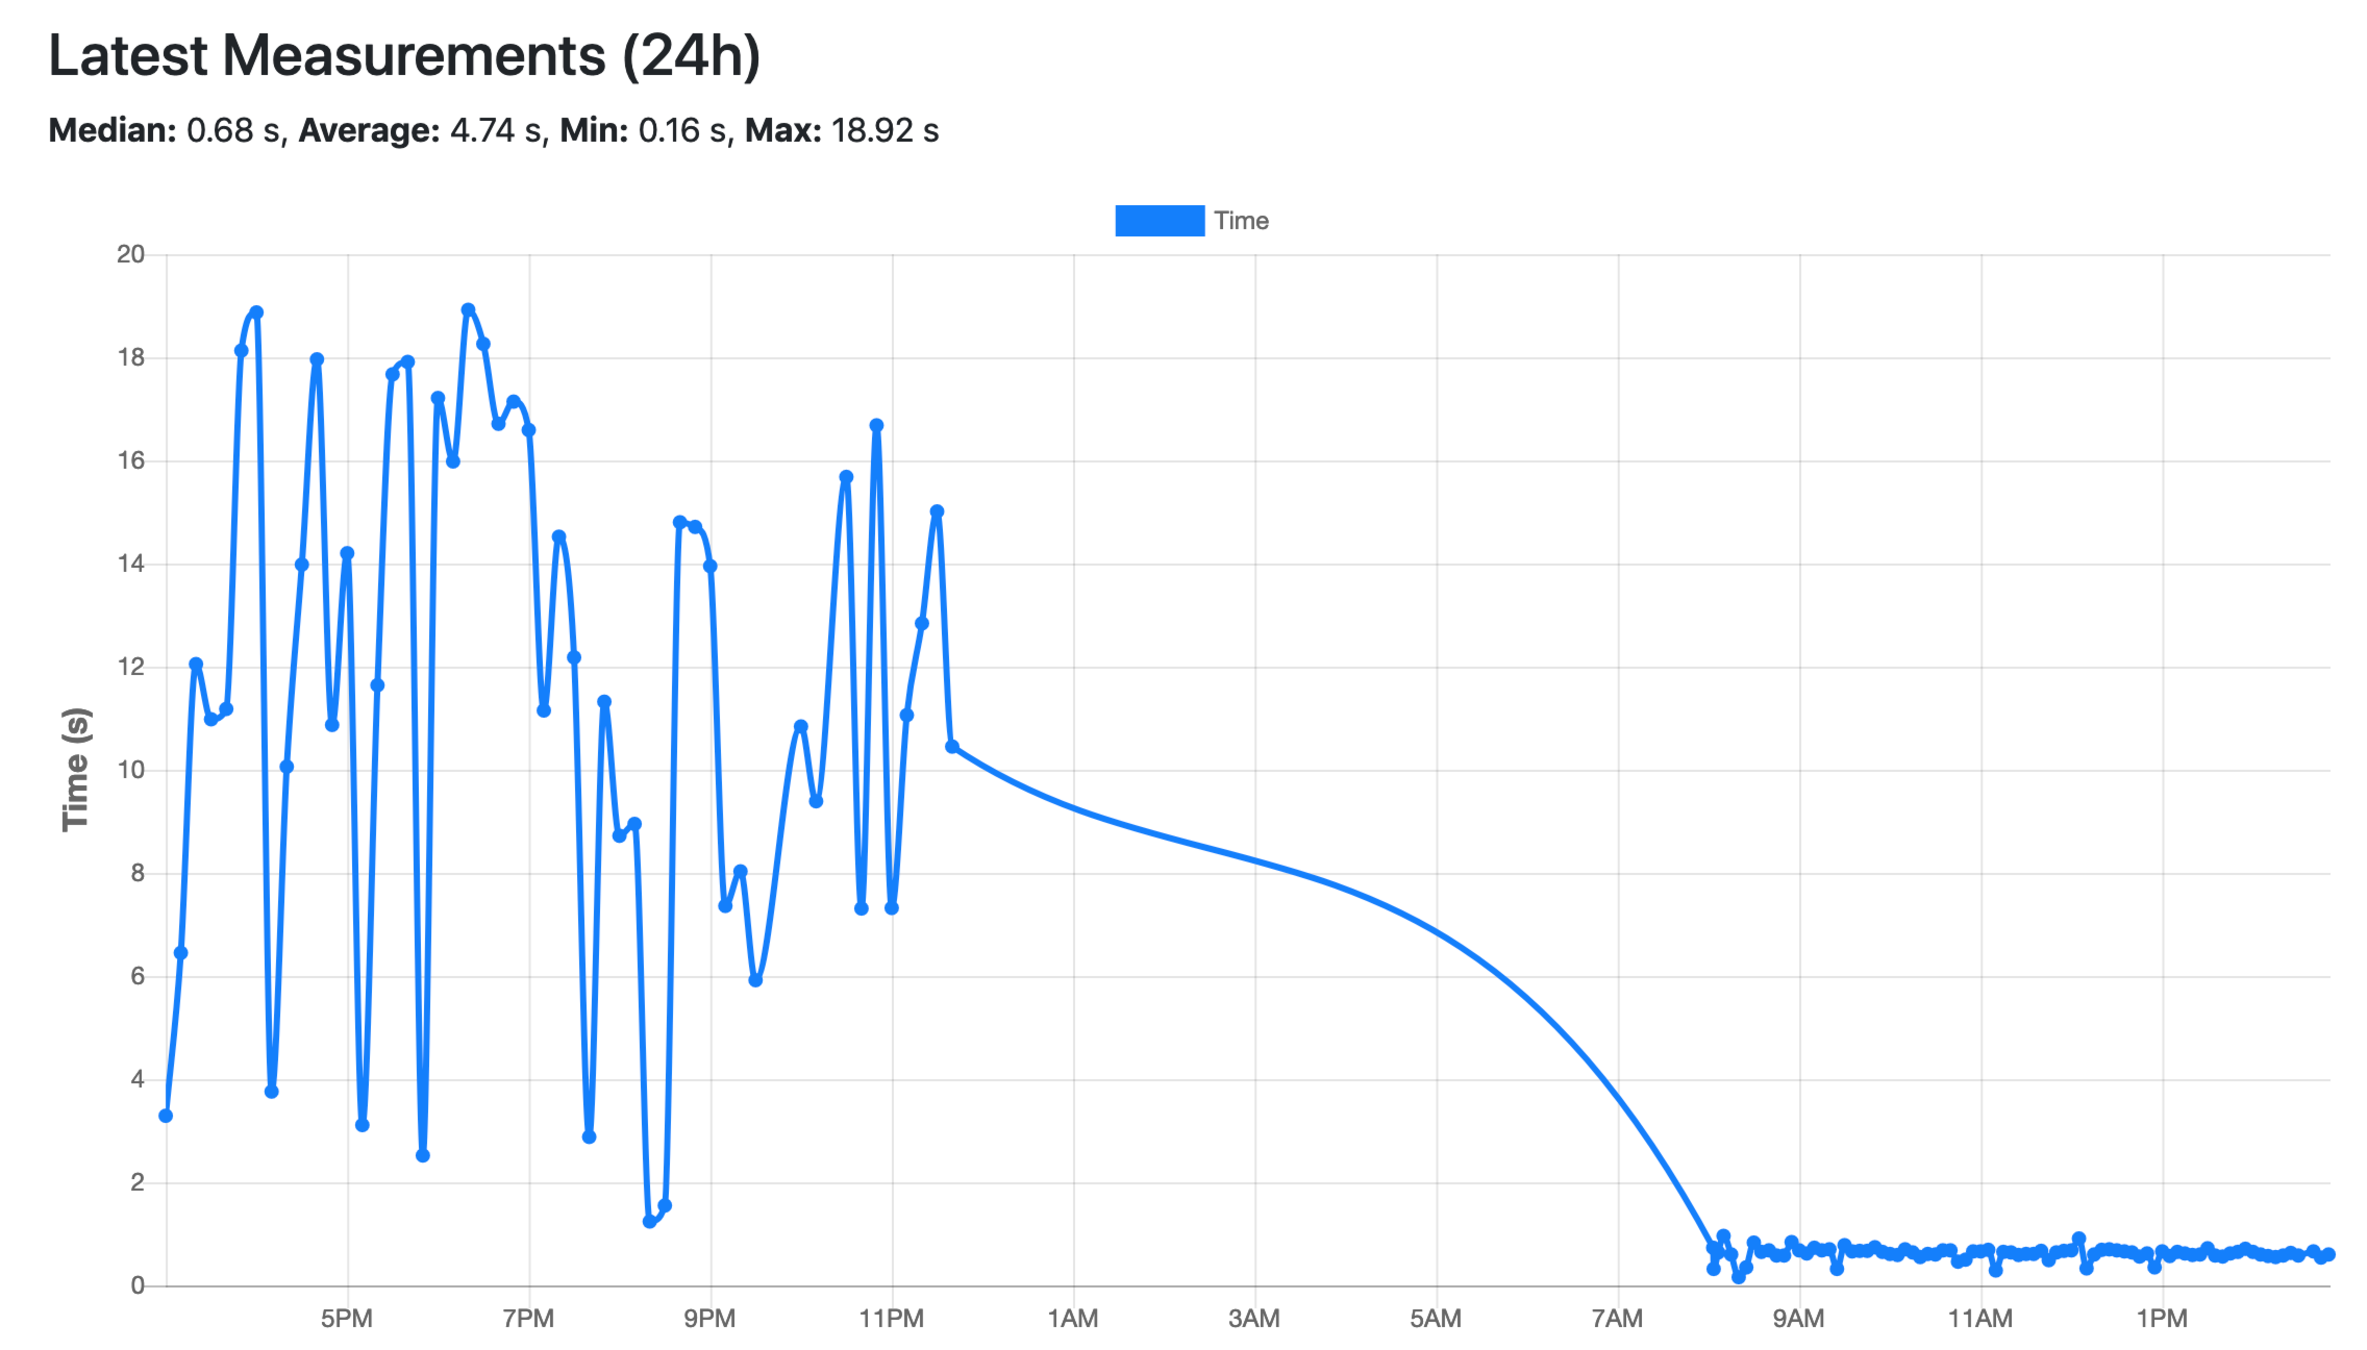
\includegraphics[width=\textwidth]{img/nano-confirmation-time.pdf}
    \caption{Improvements of transaction times after the update to V18 on February 22nd, 2019}
    \label{fig:NanoConfirmationTime}
\end{figure}
\leavevmode
\\
Although increased transaction times did play a role, the main reason Nano was not chosen for the implementation is that it wasn't built with M2M transactions in mind. To prevent spamming, i.e. attacking the network through congesting it with transactions, PoW needs to be generated in order to send or receive transactions. According to the Nano white paper\cite{nano-white-paper} an Intel Core i7-4790K processor with 4.00 GHz can handle up to 0.33 TPS. A microcontroller would not be able to generate the PoW required for the transactions in a reasonable amount of time. Instead, a dedicated server would be required for each supplier and customer, which would store the private keys and handle the transmission and reception of transactions. The micro controllers would merely communicate with said servers.
\\\\
One way to cut transaction costs is the use of off-chain transactions. As previously mentioned, these work very similarly to on-chain transactions: information like a beneficiary and value can be signed by a sender, so it can be proven where the transaction originates from. They differ from each other, as off-chain transactions, as the name suggests, are not recorded on the blockchain and therefore are feeless. A number of these off-chain transactions can be bundled in a payment channel. In the end, these transactions have to be settled on the blockchain, actually modifying the ledger and updating the balances of all participants. Thus the 2,460 transactions required during a charging period of 11 hours can be bundled into a few transactions on the blockchain, while still meeting all the requirements listed above.
\\
Ethereum was chosen for the implementation of this prototype, as it is Turing complete, therefore a payment channel can be implemented using smart contracts. The following steps briefly explain how this concept works:

\begin{enumerate}
    \item The customer places a deposit (max. purchase value) into the Smart Contract and initializes the payment channel.
    \item The customer signs an off-chain transaction and sends it to the supplier.
    \item Once the supplier receives the transaction, the delivery of electricity begins.
    \item Steps 2 \& 3 are repeated until the customer or the supplier want to discontinue the exchange.
    \item As soon as any party wants to close the payment channel, the supplier submits the offline transactions to the Smart Contract. Each party is now able to withdraw their share from the Smart Contract.
\end{enumerate}
With payment channels, the risk of the supplier is minimal, as electricity must only be provided when a valid payment was received and the customer only risks losing one transaction for the initialization of the payment channel and one off-chain transaction if no electricity is provided in return (with the values above this adds up to 0.017\euro).
\\
In total, only 4 transactions have to be made. One for the payment channel initialization, one for the settlement, and one by each party to withdraw the balances totaling all transaction costs at a couple cents.